\documentclass[11pt]{article}
\usepackage[utf8]{inputenc}
\usepackage{amsfonts}
\usepackage{amsmath}
\usepackage{float}
\usepackage{tikz}
\usetikzlibrary{trees}
\tikzset{
	sibling distance=2cm,
	every node/.style = {
		shape=rectangle,
		draw,
		align=center,
		minimum height=2em
	},
	edge from parent fork down
}

\setlength{\parindent}{0em}
\setlength{\parskip}{1em}

\usepackage{geometry}
\geometry{
  a4paper,
  total={170mm,257mm},
  left=20mm,
  top=20mm,
}

\title{Problem Sheet 5}
\author{Rowan Saunders}
\begin{document}

\begin{titlepage}
	\maketitle
\end{titlepage}

\section{Context Free Grammars and Parse Trees}
Recall the context free grammar:
\begin{align*}
	S &\to ENM \mid MNE\\
	E &\to : \mid ;\\
	N &\to \varepsilon \mid -N\\
	M &\to ( \mid ) \mid [ \mid ]
\end{align*}

\begin{itemize}
	\item Given the string $:-)$
		\begin{figure}[H]
			\centering
			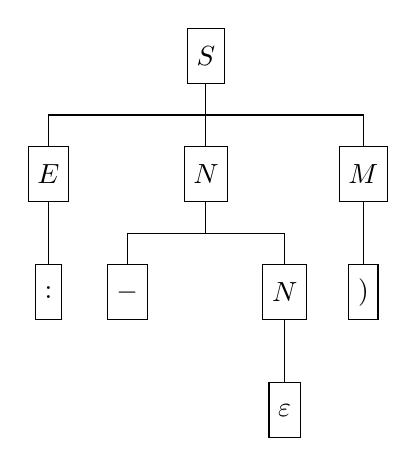
\begin{tikzpicture}
				\node {$S$}
				child { 
					node {$E$}
					child { 
						node {$:$}
					}
				}
				child {
					node {$N$}
					child {
						node {$-$}
					}
					child {
						node {$N$}
						child {
							node{$\varepsilon$}
						}
					}
				}
				child {
					node {$M$}
					child {
						node {$)$}
					}
				};
			\end{tikzpicture}
		\end{figure}
	\item Given the string $)-:$
		\begin{figure}[H]
			\centering
			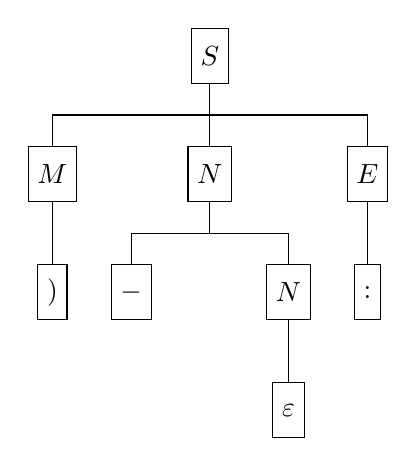
\begin{tikzpicture}
				\node {$S$}
				child {
					node {$M$}
					child {
						node {$)$}
					}
				}
				child {
					node {$N$}
					child {
						node {$-$}
					}
					child {
						node {$N$}
						child {
							node{$\varepsilon$}
						}
					}
				}
				child { 
					node {$E$}
					child { 
						node {$:$}
					}
				};
			\end{tikzpicture}
		\end{figure}
	\item Given the string $;)$
		\begin{figure}[H]
			\centering
			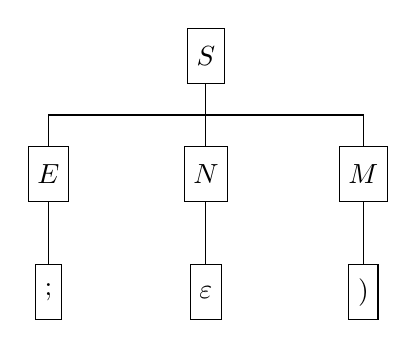
\begin{tikzpicture}
				\node {$S$}
				child { 
					node {$E$}
					child { 
						node {$;$}
					}
				}
				child {
					node {$N$}
					child {
						node{$\varepsilon$}
					}
				}
				child {
					node {$M$}
					child {
						node {$)$}
					}
				};
			\end{tikzpicture}
		\end{figure}
	\item Given the string $:--]$
		\begin{figure}[H]
			\centering
			\begin{tikzpicture}
				\node {$S$}
				child { 
					node {$E$}
					child { 
						node {$:$}
					}
				}
				child {
					node {$N$}
					child {
						node {$-$}
					}
					child {
						node {$N$}
					  child {
						  node {$-$}
					  }
						child {
							node {$N$}
							child {
								node{$\varepsilon$}
							}
						}
					}
				}
				child {
					node {$M$}
					child {
						node {$]$}
					}
				};
			\end{tikzpicture}
		\end{figure}

\end{itemize}

The Grammar is unambiguous. This is because there is only one possible parse
tree for every string in the language. 

\end{document}


